Au démarrage du choix de la position d'un nouveau on a un tableau a double entrée avec des cases déjà occupées par d'autre pions. Les cases libres sont représentées par des 0 tandis que les cases occupées par des pions sont notées avec des X.

\begin{center}
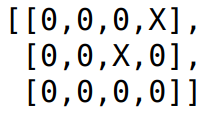
\includegraphics[scale=0.75]{image/Plateau jeu normal.png}
\end{center}


On va transformer ce tableau a double entrés en un tableau a une entrée (pour imager, il n'y a pas création réelle de ce tableau). En réalité ce nombre est directement convertie en deux valeur lisible et existante dans le tableau a double entré initial.

\begin{center}
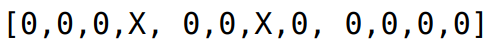
\includegraphics[width=\textwidth]{image/Plateau jeu en ligne.png}
\end{center}

En partant du principe que nous avons obtenus ce tableau a une dimension on va pouvoir savoir combien de cases sont encore libres. On va donc calculer ce nombre de cases restantes et choisir un nombre aléatoire entre 0 et le nombre de cases libres. On peux voir sur l'image suivante en rose les éléments dont leur index a potentiellement été choisie.

\begin{center}
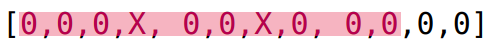
\includegraphics[width=\textwidth]{image/Plateau jeu en ligne choix nombre.png}
\end{center}


On va ensuite partir de l'index 0 et remonter jusqu’à l'indexe de la nouvelle case pour vérifier que la case choisie n'est pas déja occupé par un autre pion.

\begin{center}
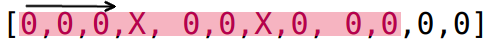
\includegraphics[width=\textwidth]{image/Plateau jeu en ligne choix nombre direction.png}
\end{center}


Ici on peux remarquer qu'un pion est présent sur cette case et pour éviter qu'un autre pion ne s'y trouve on ajoute 1 a l'index de tout les cas possibles qui on un index superieur ou égale a la position d'un pion occupé. En fessant cela on modifie aussi l'index final de la boucle qui va faire une itération supplémentaire. On peut mieux observer ce décalage sur l'image suivante.

\begin{center}
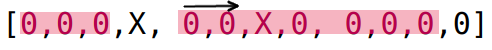
\includegraphics[width=\textwidth]{image/Plateau jeu en ligne choix nombre direction 2.png} 
\end{center}

On a la même situation que précédemment donc tous les index possiblement choisi qui son supérieurs ou égales a celui de la case déjà prise, on leur ajoute 1.

\begin{center}
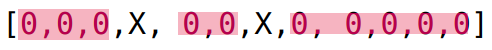
\includegraphics[width=\textwidth]{image/Plateau jeu en ligne choix nombre direction 3.png} 
\end{center}

On vérifie toujours la case sur laquelle est la position du nouveau pion et si elle est déjà occupé on ajoute 1 jusqu’à ce qu'elle soit vide.

Enfin la position du pion va être écrite dans le tableau a double entrées en transformant ce nombre en deux nombres pour le plateau de jeu.
Je rappelle que les positions en rose sont les positions que peux prendre le pion dont l'index est aléatoirement choisie.

\begin{center}
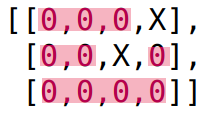
\includegraphics[scale=0.75]{image/Plateau jeu normal final.png}
\end{center}